
\documentclass[tikz,margin=5mm]{standalone}
\usetikzlibrary{circuits.ee.IEC}

\begin{document}
	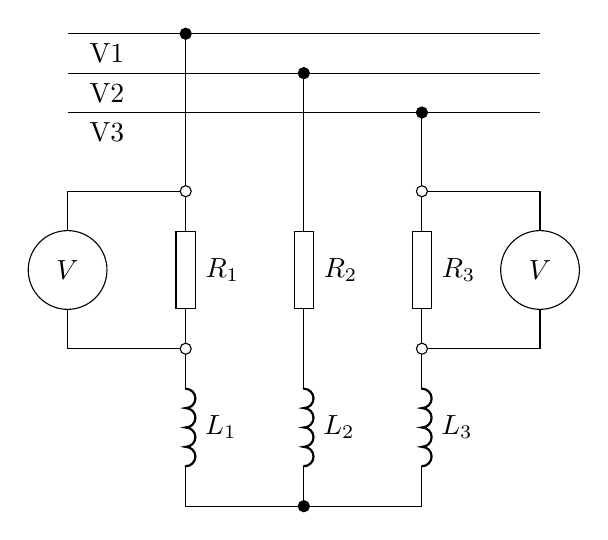
\begin{tikzpicture}[circuit ee IEC, circuit symbol lines/.style={draw,thick}]
	
	%Matrix
	\def\spaltenabstand{1.5cm}
	\def\zeilenabstand{0.5cm}
	\def\zeilenzahl{15}
	\def\spaltenzahl{7}
	\foreach \i in {1,...,\zeilenzahl}
	\foreach \j in {1,...,\spaltenzahl}
	{
		\coordinate (S-\i-\j) at ({(\j-1)*\spaltenabstand},{-(\i-1)*\zeilenabstand});
		%\node at (S-\i-\j){+}; % Orientierungshilfe
	}
	
	%Schaltung
	\draw (S-8-2) to  [resistor={info=$R_1$}](S-10-2); 
	\draw (S-12-2) to  [inductor={info=$L_1$}](S-14-2);
	
	\draw (S-8-3) to  [resistor={info=$R_2$}](S-10-3); 
	\draw (S-12-3) to  [inductor={info=$L_2$}](S-14-3);
	
	 \draw (S-8-4) to  [resistor={info=$R_3$}](S-10-4); 
	 \draw (S-12-4) to  [inductor={info=$L_3$}](S-14-4);
	 
	 
	%\draw (S-4-2)[fill=white] circle [radius=15pt];
	\node[draw,circle,minimum size=1cm,inner sep=0pt] at (S-9-1){$V$};
	\node[draw,circle,minimum size=1cm,inner sep=0pt] at (S-9-5){$V$};
	\node[] at (0.5,-1.25) {V1};
	\node[] at (0.5,-1.75) {V2};
	\node[] at (0.5,-2.25) {V3};
%	\node[draw] at (0,0) {test}
	%Leiterbahnen
	
	\draw 
	(S-8-2)--(S-7-2)--(S-3-2)
	(S-12-2)--(S-10-2)
	(S-3-1)--(S-3-5)
	
	(S-8-3)--(S-7-3)--(S-4-3)
	(S-12-3)--(S-10-3)
	(S-4-1)--(S-4-5)
	
	(S-8-4)--(S-7-4)--(S-5-4)
	(S-12-4)--(S-10-4)
	(S-5-1)--(S-5-5)
	
	(S-7-2)--(S-7-1)--(S-8-1)
	
	(S-11-2)--(S-11-1)--(S-10-1)
	
	(S-7-4)--(S-7-5)--(S-8-5)
	
	(S-11-4)--(S-11-5)--(S-10-5)
	
	(S-14-2)--(S-15-2)--(S-15-3)--(S-14-3)
	(S-15-3)--(S-15-4)--(S-14-4);
	
	Knotenpunkte, Klemmen (extra zeichnen, so keine Überschneidungen)
	\foreach \p in {S-11-2,S-11-4,S-7-2,S-7-4}
	\draw[fill=white] (\p) circle [radius=2pt];
	
	\foreach \p in {S-15-3,S-3-2,S-4-3,S-5-4}
	\draw[fill] (\p) circle [radius=2pt];
	
	\end{tikzpicture}
\end{document}